\appendix

\section{Implementation Details}
\label{appendix:detail}
\paragraph{Language Modeling}
For language modeling experiments, we train OPT-1.3B, OPT-2.7B, and RedPajama-3B with the next token prediction objective. The loss is computed on all tokens except for newly added \textit{<CL>} and \textit{<CR>} tokens. For tokens right before \textit{<CL>} and \textit{<CR>}, we adjust their ground-truth label to be tokens right after 
the corresponding \textit{<CL>} and \textit{<CR>} tokens.

The trainable parameters for all LLMs include two token embeddings of \textit{<CL>} and \textit{<CR>}, and LoRA modules applied to all attention layers. The rank of weight matrices of LoRA is set to 16. The percentage of trainable parameters takes about 5\% of the total parameters of the LLM.
We use AdamW~\cite{adamw} optimizer with a 2e-5 learning rate. The batch size is set to 12 and the maximum sequence length during training is set to 256 due to the limited computation budget. The implementation is based on Huggingface transformers~\cite{wolf-etal-2020-transformers} library and all experiments are conducted using a single RTX 3090 GPU.
\paragraph{Open-ended Document Generation}
For open-ended document generation, we use nucleus sampling with top p$=$0.9. Due to the randomness induced by sampling, we perform 8 times nucleus sampling for each compressed prefix and report the average evaluation metrics adopted in the main paper. 
This helps reduce variance and ensures a more reliable evaluation result.
% \paragraph{Inference-time Compression} Given a text piece as the prefix, we apply the same input transformation strategy used during training to reach a specified compression ratio. To realize perceivable memory and computation reduction, the key-value cache of tokens enclosed by sentinel tokens is freed from GPU in a progressive manner~(e.g., using a for-loop) if the original prefix is too long to fit into GPU. Otherwise, we just feed the transformed prefix through the model in one go.
\section{Generalization Ability of KV Compression}
\begin{figure}[th]
	\centering
	\scalebox{0.33}{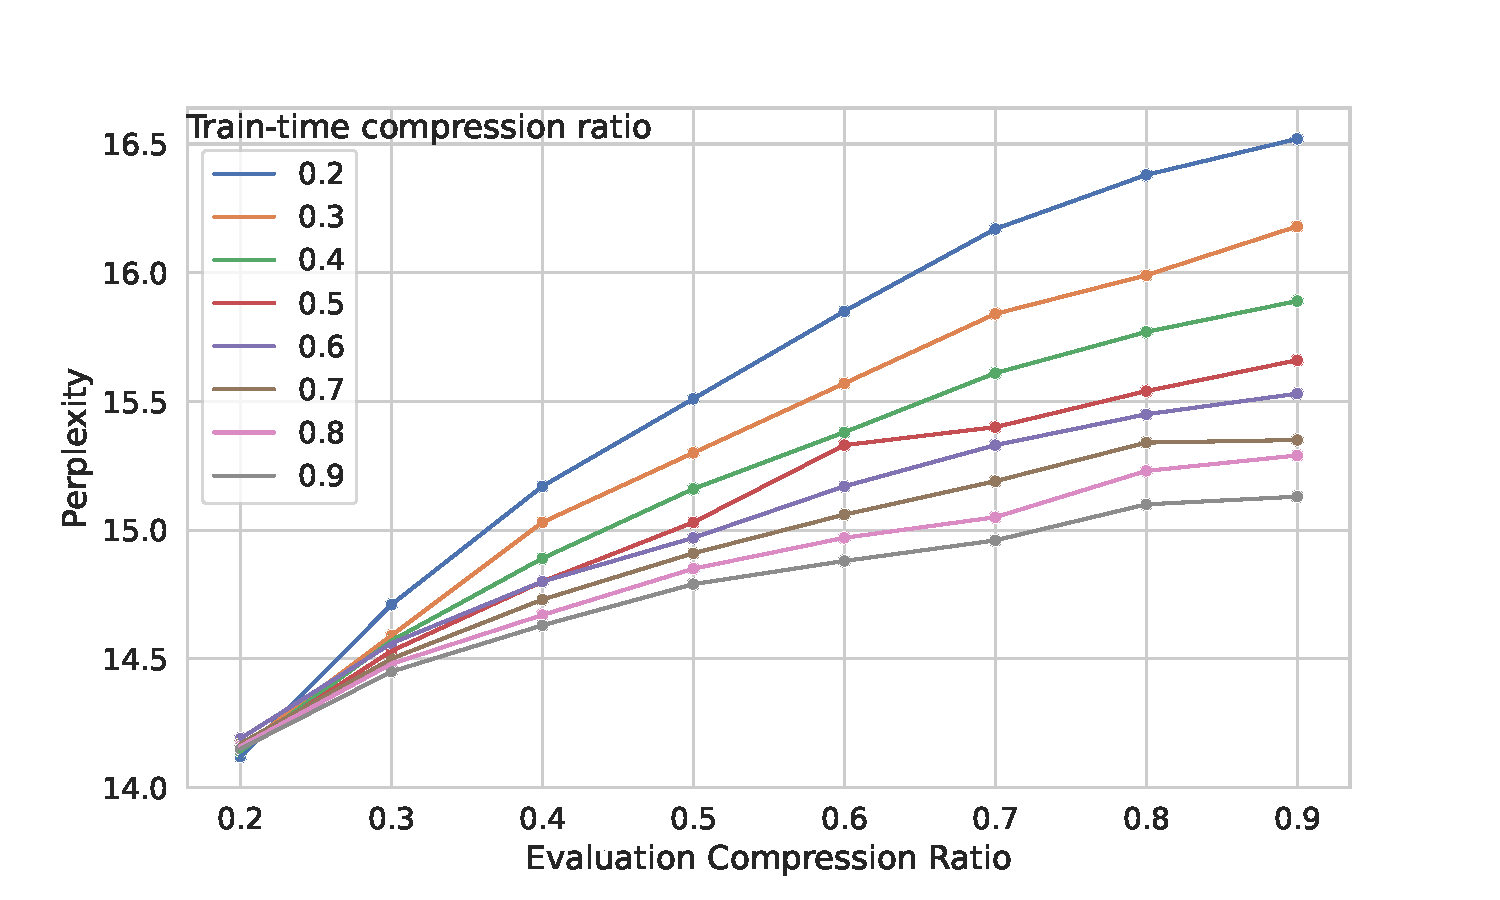
\includegraphics{./figures/extrapolation.pdf}}
	\caption{Generalization performance of different train-time compression ratios. }
	\label{fig:extrapolation}
\end{figure}
\label{appendix:extrapolation}
In our proposed KV Compression, an LLM is trained on transformed data in which the percent of tokens surrounded by sentinel tokens takes a specified ratio of the total number of tokens. Here we study the generalization performance of different train-time compression ratios and explore the best practice. 
We visualize the perplexity of RedPajama-3B trained with different compression ratios at varying test-time compression ratios. 

\figref{fig:extrapolation} illustrates the results. We can see that training with a higher compression ratio always results in better generalization ability across various test-time compression ratios. The 
reason is that, at a small compression ratio, language models can sometimes exploit limited local context and can still reliably predict the next token. In this case, the sentinel tokens are not guaranteed to acquire the desired context compression ability. When the majority of context is not allowed to be attended to, the sentinel tokens are forced to cultivate enough compression ability in order to 
minimize the loss function.

\section{Memory Usage with Varied Compression Ratio}
\begin{figure}[th]
	\centering
	\scalebox{0.333}{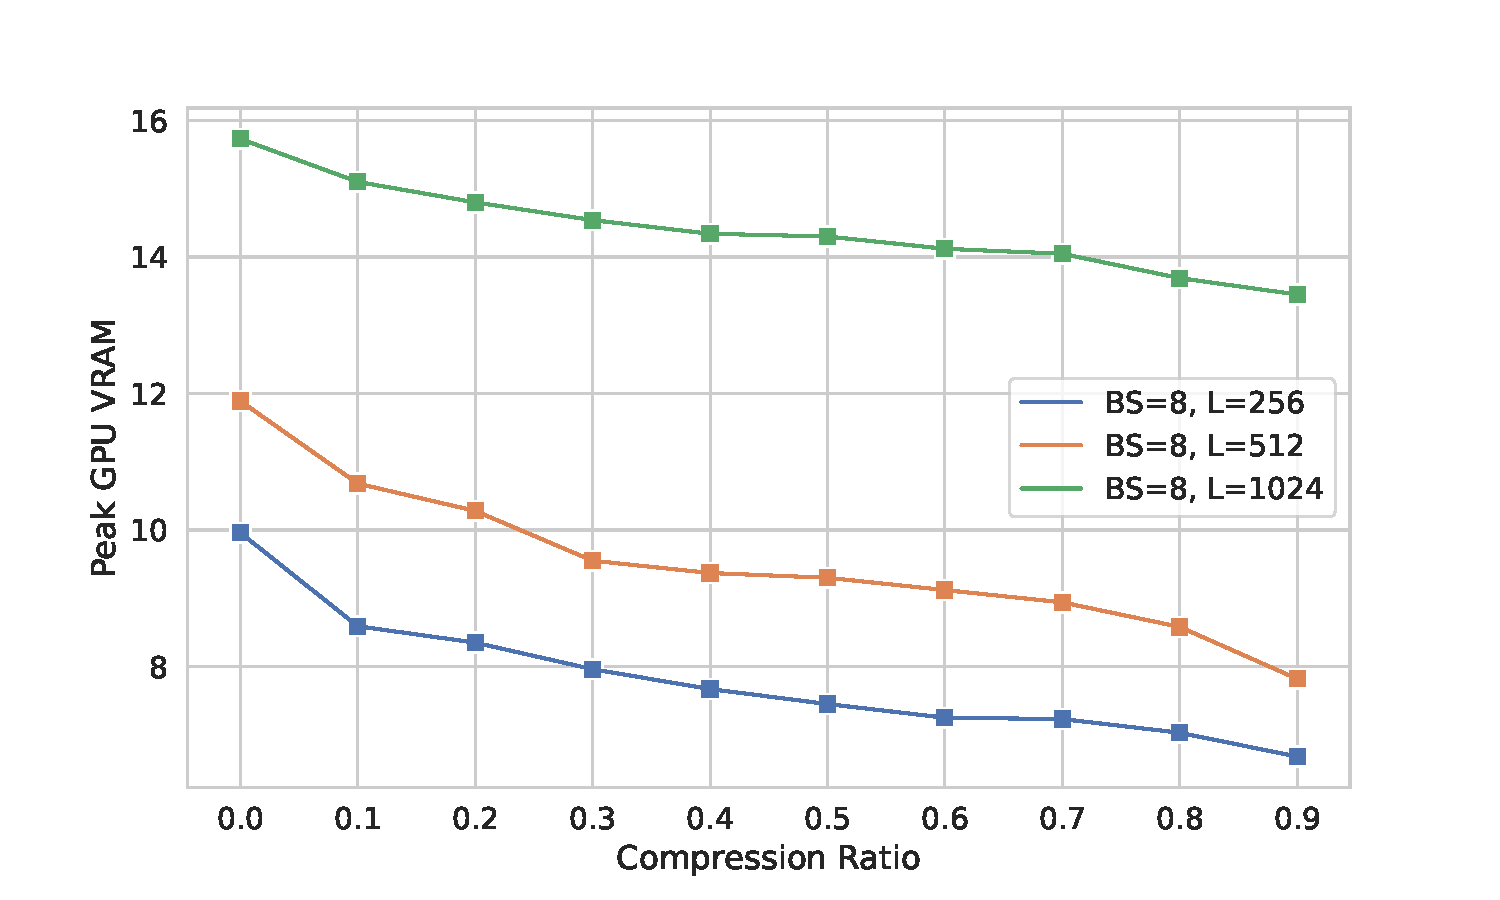
\includegraphics{./figures/redpajama3b_memory.pdf}}
	\caption{Peak cached memory profiled using Pytorch when using RedPajama-3B to produce a 100-token continuation for variable-length prefixes.}
	\label{fig:memory}
\end{figure}
We have shown that context compression confers decent improvement in system throughput, especially for moderate-sized GPUs. Here we report detailed memory usage assuming a practical scenario similar to multi-turn dialogue: the 
prefix length~(length of historical dialogue) gradually increases, and the model is asked to output a response of roughly 100 tokens. To maximize the throughput of dialogue service, we assume the model is simultaneously generating responses for multiple instances, i.e., a batch size larger than one.

\begin{figure*}[th]
	\centering
	\scalebox{0.318}{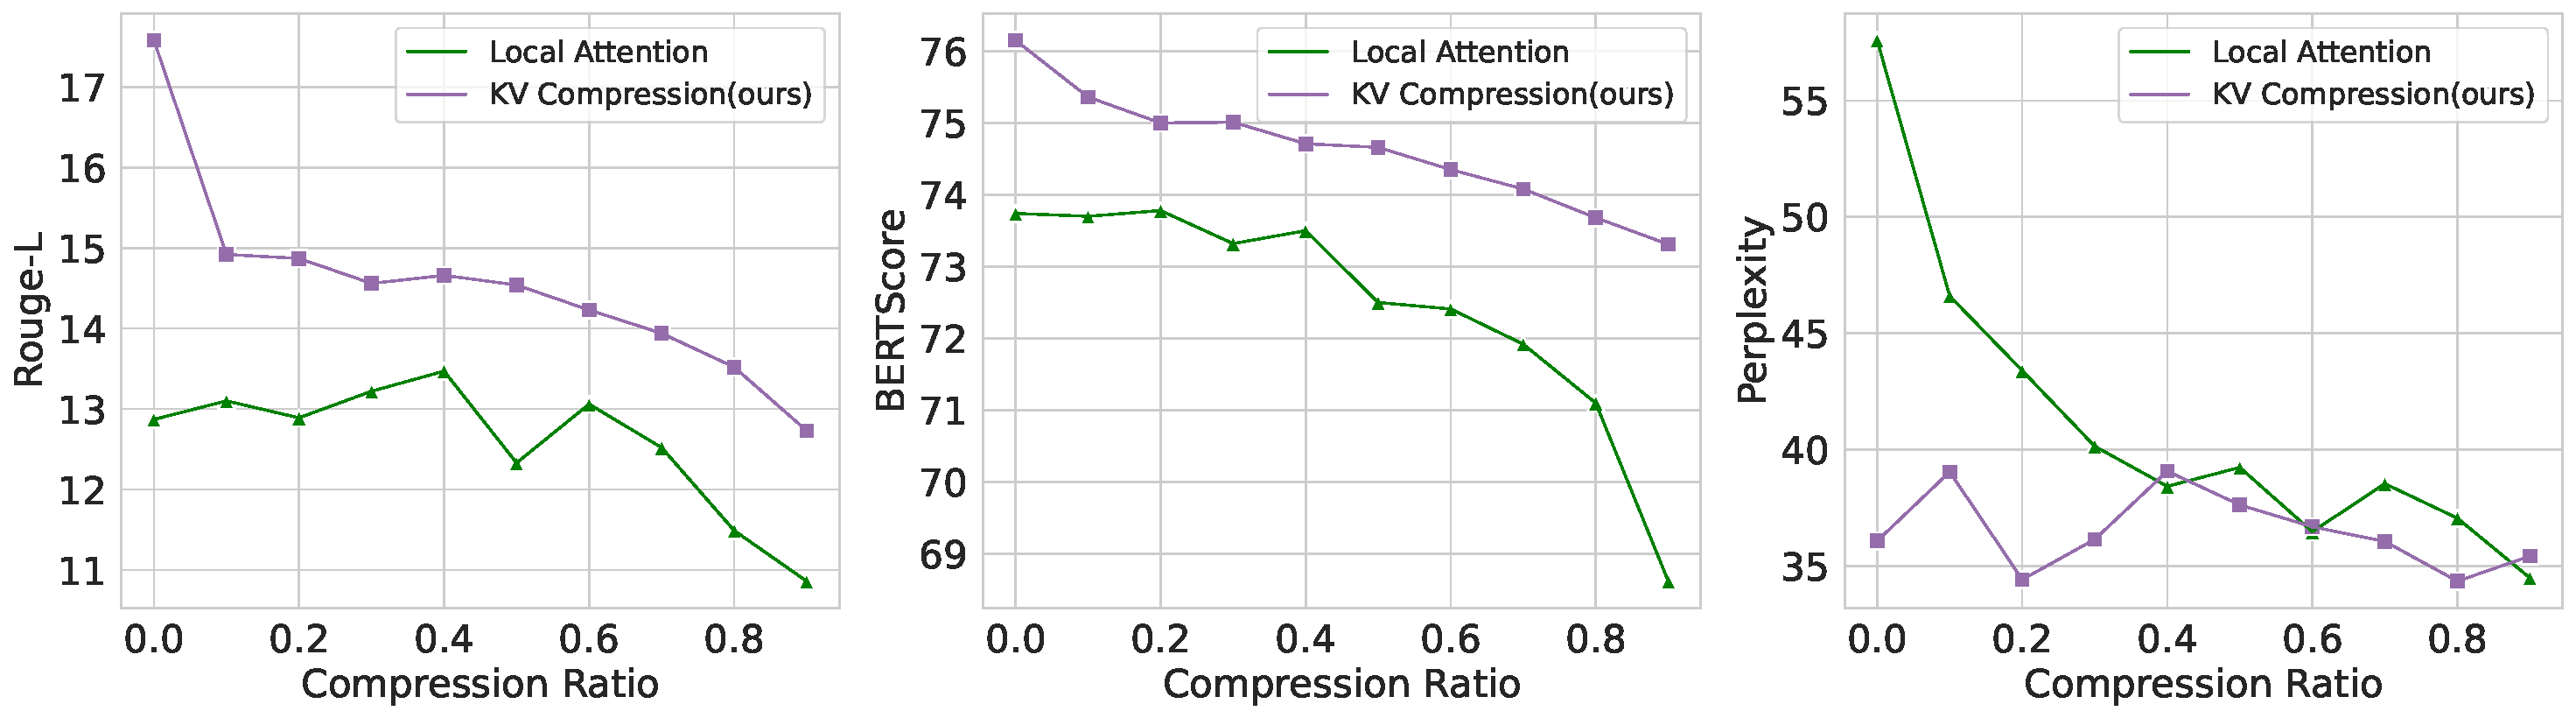
\includegraphics{./figures/opt1b_all.pdf}}
	\caption{OPT-1B on open-ended generation on 200 sampled C4 documents. Generation quality is measured by fluency~(perplexity), n-gram matching~(ROUGE-L), and semantic similarity~(BERTScore).}
	\label{fig:opt1ball}
\end{figure*}
The visualized memory usage is shown in \figref{fig:memory}. Context compression is able to reduce more than 3GB of peak cached GPU memory. In practice, this translate to the feasibility of generating more tokens for a single instance and enabling more instances in parallel.
\section{Open-ended Generation Results of OPT}
\figref{fig:opt1ball} summarizes the results of OPT-1B on open-ended document generation. Compared to that of Redpajama-3B~(\figref{fig:open_ended}), the generation quality of OPT-1B is substantially lower. Comparing different context compression methods, KV 
Compression performs uniformly better across all three evaluation metrics.
\label{appendix:memory}